


\chapterauthor{Jeferson J. Lima}{Departamento de Informática (DAINF) \\Universidade Tecnológica Federal do Paraná (UTFPR)}


% \chapter{Contexto Histórico}

% \section{Introdução}\label{intro-ch0}


\chapter{Revisão de Conceitos}

% \section{Introdução}\label{intro}

% A component part for an electronic item is
% manufactured at one of three different factories, and then delivered to
% the main assembly line.Of the total number supplied, factory A supplies
% 50\%, factory B 30\%, and factory C 20\%. Of the components
% manufactured at factory A, 1\% are faulty and the corresponding
% proportions for factories B and C are 4\% and 2\% respectively. A
% component is picked at random from the assembly line. What is the
% probability that it is faulty?

\section{Primeiros passos com a Linguagem Python}\label{python}

É comum quando estamos iniciando no mundo da matemática, nos depararmos com a necessidade de desenhar gráficos, algo como a figura baixo:

\begin{figure}
    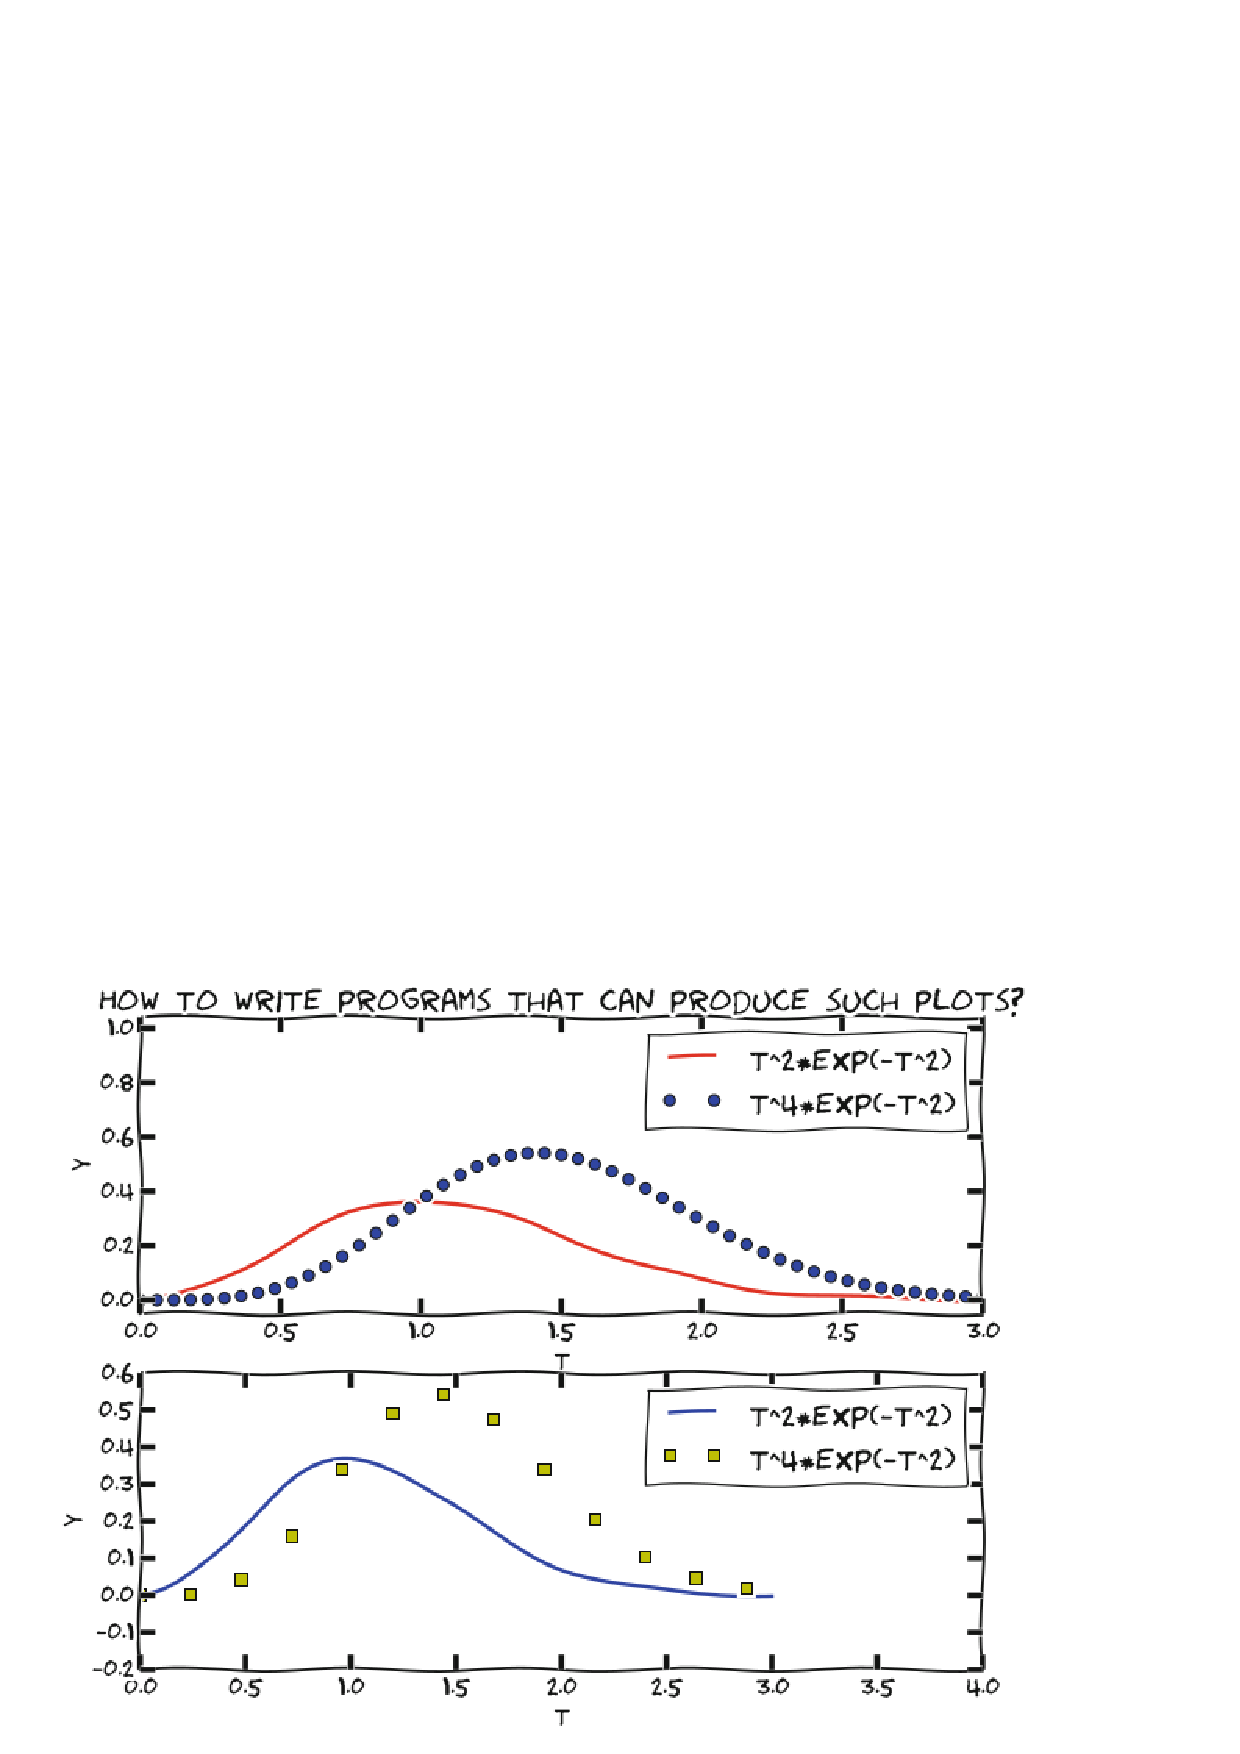
\includegraphics[width=250pt, height=200pt]{chapters/chapter0/figures/manual_graph.png}
    \caption[Desenhando Gráficos Manualmente]{Desenhando Gráficos Manualmente}
\end{figure}

Não somente nas engenharia os profissionais necessitam das habilidades de manipular e exibi-los dados graficamente,
a maioria das pessoas tem experiencias em softwares como Microsoft Excel, Libreoffice Calc, entre outras ferramentas dedicadas.
No entanto, essa interação geralmente é bastante simples, com alguns cliques é possível gerar diversos gráficos para visualização dos dados.

Porém, dada a característica dos dados a serem plotados, faz-se necessário um nível de customização maior, surgindo a necessidade.

Python é uma excelente linguagem para iniciantes, bem como usuários avançados, pois possui uma sintaxe simples e clara. Outro ponto
forte é as bibliotecas de python que apresenta diversas opções para processamento e visualização de dados. Destaca-se inicialmente aqui, duas
bibliotecas que serão utilizadas no inicialmente, a biblioteca para processamento numérico \textbf{numpy}, biblioteca \textbf{scipy} com diversas
funções da área de ciência da computação e \textbf{matplotlib} para visualização dos dados.
\subsection{Instalação do Python}

Para estudar desta matéria, você precisa de uma instalação do Python que atenda ao propósito de aula. A maneira mais rápida de obter uma instalação útil do Python em seu computador Windows ou Mac,
é baixar e instalar o Anaconda (https://www.anaconda.com/). Em muitas distribuições de linux, o Python já é nativo,
caso não seja, aconselha-se a instalação pelo terminal utilizando linha de comando.

\begin{lstlisting}
    $ sudo apt-get install python3
\end{lstlisting}

A versão de Python2 está obsoleta desde janeiro de 2020, sendo assim, nem suporte desde então. Por este motivo aconselha-se
a instalação de Python3.

A instalação de uma biblioteca do Python pode ser dada através do comando:
\begin{lstlisting}
    $ sudo python3 -m pip install numpy
\end{lstlisting}

Há diversas opções de serviços online, como a ferramenta Colab do Google, onde disponibiliza opções com recursos computacionais interessantes,
a uma conta google são oferecidas três opções de hardware, Máquina sem GPU, com GPU e uma Máquina com TPU.

\subsection{Problemas Numéricos com Python}

Para o nosso primeiro exemplo de problema numérico utilizando a linguagem Python, vamos fazer uso da expressão do grafico abaixo.

\begin{equation*}
    y = t^2\exp(-t^2)
\end{equation*}

Neste momento, teremos que recorrer a algumas funções da biblioteca \textbf{numpy}, como \textbf{numpy.exp} e \textbf{numpy.linspace} para gerar um vetor de tempo $t$.

\begin{lstlisting}
    ## importando bibliotecas
    from numpy import exp, linspace
    ## Definindo a funcao
    def yf(t):
        return t**2*exp(-t**2)

    # vetor t, inicio em 0 e fim em 3
    #   com 50 elementos
    t = linspace(0,3,50)

    y = yf(t)
\end{lstlisting}

Assim a variável $y$ recebe $y_f(t)$.

\subsubsection{Plotando Dados}

Dando continuidade ao exemplo anterior, apresentamos aqui outra biblioteca do python, a  \textbf{matplotlib} para visualização dos dados.
Considerando o exemplo acima, temos:

\begin{lstlisting}
    ## importando bibliotecas
    from numpy import exp, linspace
    ## Definindo a funcao
    def yf(t,n):
        return t**n*exp(-t**2)

    # vetor t, inicio em 0 e fim em 3
    #   com 50 elementos
    t = linspace(0,3,50)

    y1 = yf(t,2)
    y2 = yf(t,4)

    # importando o modulo pyplot e renomeando como plt
    import matplotlib.pyplot as plt

    plt.plot(t,y1)
    plt.plot(t,y2, "o")
    plt.xlabel("t")
    plt.ylable("y")
    plt.legend(["T^2*EXP(-T^2)", "T^4*EXP(-T^2)"])
\end{lstlisting}

O resultado esperado será:

\begin{figure}[htb]
    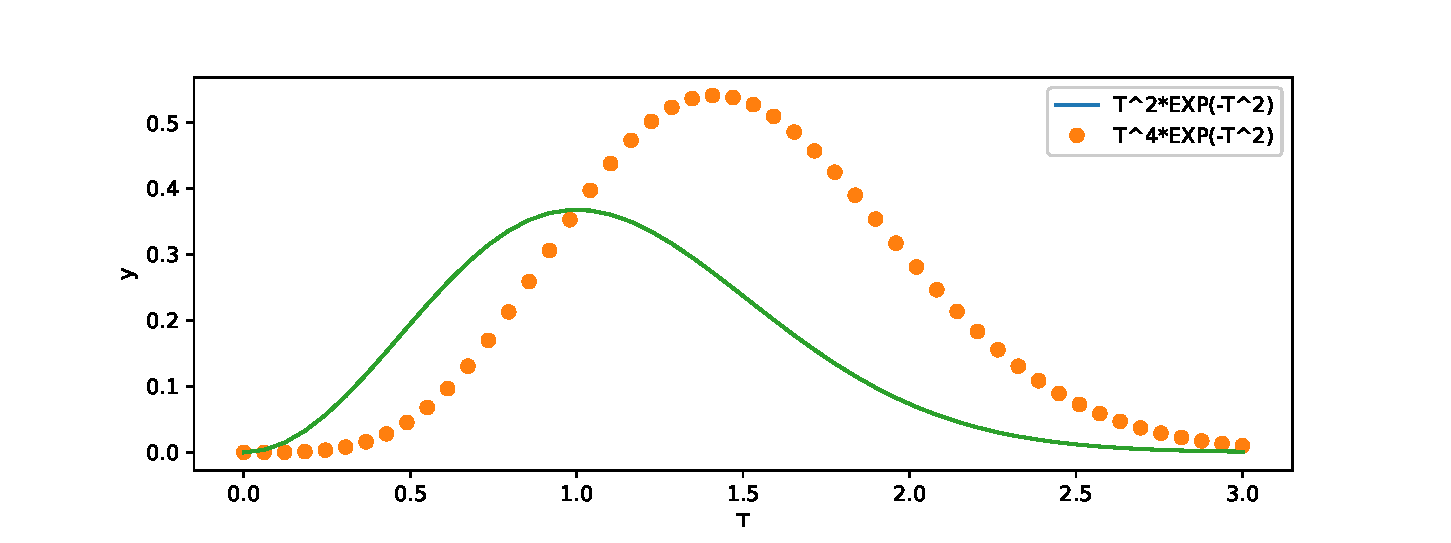
\includegraphics[width=300pt]{chapters/chapter0/figures/python_graph.eps}
    \caption[Desenhando Gráficos Manualmente]{Matplotlib Gráficos}
\end{figure}

A uma série de customizações que podem ser feitas no gráfico, como escrever a legenda em latex, mudança de cores, etc ... Para mais informações consulte a documentação do 
\textbf{matplotlib} na internet.

\subsubsection{Simulação numérica de Sistemas Dinâmicos}

\begin{VF}
    ``Um sistema dinâmico contínuo é um sistema dinâmico cujo estado evolui ao longo do espaço de estado continuamente de acordo com uma regra fixa.''
    
    \VA{Jaime E. Villate}{Introdução aos sistemas dinâmicos, 2007}
    \end{VF}

    Para entender melhor como resolver numericamente um sistemas dinâmicos utilizando uma linguagem de programação, primeiro precisamos recorrer ao problema.

    Aqui será apresentado um problema simples, onde deseja se saber a velocidade de um veículo, considerando limitações impostas pelo seu modelo dinâmico, O veículo está sobre uma superfície plana em condições de rolagem... então é aplicado uma força de tração $u$ ("um empurrão") no sentido do seu movimento, $b$ será o coeficiente de atrito e $m$ a massa.

\begin{figure}[htb]
    \includegraphics[width=200pt]{chapters/chapter0/figures/cruise_control_schematic.png}
    \caption[Desenhando Gráficos Manualmente]{Matplotlib Gráficos}
\end{figure}

Deve-se agora listar as forças com base na física do sistema.

\begin{equation*}
    m\dot{v}+bv=u
\end{equation*}

Substituindo $v$ por $\dot{x}$:

\begin{equation*}
    m\ddot{x}+b\dot{x}=u
\end{equation*}

sendo $x$, posicionamento, $\dot{x}$ velocidade e $\ddot{x}$ aceleração, temos então a função de espaço de estados:

\begin{equation}\label{eq:car}
    \frac{d}{dt}\begin{bmatrix} x_0 \\ x_1 \end{bmatrix} = 
    \begin{bmatrix} 1 & 0\\ -\displaystyle\frac{b}{m} & +\displaystyle\frac{1}{m} \end{bmatrix}
    \begin{bmatrix} x_1 \\ u \end{bmatrix}    
\end{equation}

A solução numérica de Eq. \ref{eq:car} é obtida através de um método de integração, em Python a biblioteca \textbf{scipy} traz os diversos métodos de integração, a função responsável por chamar o integrador é \textbf{odeint}.

\begin{lstlisting}
    import numpy as np
    import matplotlib.pyplot as plt
    from scipy.integrate import odeint

    ## Definindo a funcao carro
    def car(x,t):
        m = 2000
        b = 240
        u = 100
        # inicializando vetor derivadas
        dx = np.zeros(2,)
        dx[0] = x[1]
        dx[1] = 1/m*(-b*x[1]+u)
        return dx

    # vetor t, inicio em 0 e fim em 3
    #   com 100 elementos
    t = np.linspace(0,10,100)
    # condicoes iniciais
    x0 = [0,0]

    # integrador
    x = odeint(car, x0, t)

    # plotando os valores
    plt.plot(t,x[:,0],t,x[:,1])
    plt.xlabel("t")
    plt.legend(["Posicao", "Velocidade"]) 
\end{lstlisting}
 
A solução numérica pode ser vista pelo gráfico abaixo:

\begin{figure}[htb]
    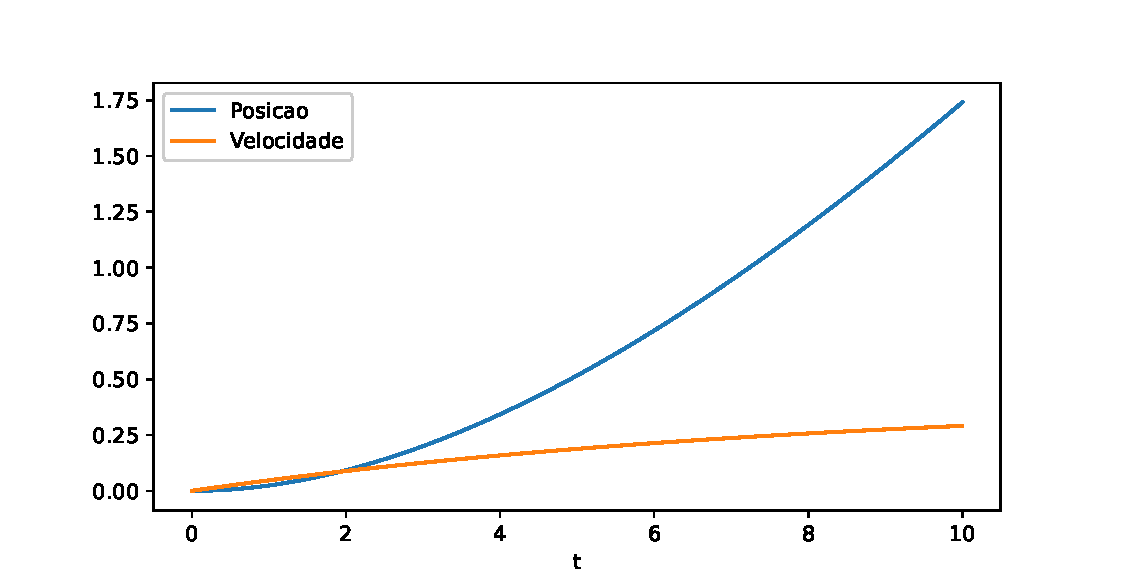
\includegraphics[width=300pt]{chapters/chapter0/figures/exercice_car.eps}
    \caption[Modelo Dinâmico Carro]{Gráfico velocidade e Posicionamento Carro}
\end{figure}

O sistema apresentado possui apenas dois estados, no entanto, sistemas de maior ordem podem ser
simulados utilizando os métodos de integração, como será visto no próximo capítulo.

\begin{shortbox}
    \Boxhead{Exercício de Fixação}
    Com base no sistema do robô demonstrado acima, escreva um programa que simule a situação onde o robô é inicializado em uma rampa com angulo de $\theta=30$ graus, lembre que ele sob da força gravitacional $G=\sin(\theta)mg$, onde $m$ é a massa e $g$ é a
    força gravitacional. Qual vai ser a velocidade e posicionamento final do robô após decorrido 10 segundos. Parâmetros: Força de tração $u=8\text{Nm}$,
    coeficiente de atrito $b=2$ e massa $m=3$.
    \begin{center}
        Resposta:

        \qrcode[height=0.5in]{Posicionamento, Velocidade: -2.0704, -0.2.432}
\end{center}

\end{shortbox}

\subsubsection{Biblioteca Simbólica}

Em algumas situações, faz se interessante utilizar ferramentas para facilitar e/ou simplificar a solução de sistemas de equações. Neste caso utilizaremos a biblioteca \textbf{sympy}, que possui várias ferramentas para solução de equações dinâmicas.

Vamos a um exemplo:

\begin{lstlisting}
    from sympy import *

    # definindo x como uma variavel
    x = symbols('x')
    eq = (sin(x)**2 + cos(x)**)**2

    # expandir equacao eq
    expand(eq)
    # >> sin(x)**4 + 2*sin(x)**2*cos(x)**2 + cos(x)**4

    # simplificar equacao eq
    simplify(eq)
    # >> 1

\end{lstlisting}

Para memorizar o uso da ferramenta de solução de equações simbólicas, vamos a alguns exercícios de fixação.

\begin{shortbox}
    \Boxhead{Exercício de Fixação}
    \begin{enumerate}
        \item  Usando o função \textbf{solve(eq,x)} encontre a solução da função quadrática $ax^2+bx+c=0$.
        \begin{center}
            Solução:

\qrcode[height=1in]{
x = symbols('x')
a = symbols('a')
b = symbols('b')
c = symbols('c')
eq2 = a*x**2+b*x+c
solve(eq2, x)
# >>[(-b + sqrt(-4*a*c + b**2))/(2*a), -(b + sqrt(-4*a*c + b**2))/(2*a)]}
\end{center}

    \item Sendo $x(t)$ uma função no tempo, use o comando \textbf{x = Function('x')} para definir a função $x$ e $t$ como 
    uma variável simbólica. Como o comando \textbf{dsolve(eq, x(t))} ache a solução da equação $\displaystyle\frac{dx(t)}{dt}+x(t)=0$
    \begin{center}
        Solução:

\qrcode[height=1in]{
x = Function('x')
t = symbols('t')
eq = diff(x(t), t) + x(t)
dsolve(eq, x(t))
eq2 = a*x**2+b*x+c
dsolve(eq2, x)
# >>Eq(x(t), C1*exp(-t))}
\end{center}

\end{enumerate}
\end{shortbox}

\section{Rotação, Translação e Transformação Homogênea}\label{rotacao}
 
Para representação de posicionamento e orientação de um sistema de coordenadas faz se necessário seguir a metodologia do sistema universal de coordenadas.

De acordo com \cite{craig2005introduction} uma vez estabelecido o sistema de coordenada como um vetor de posição $\mathbb{R}^{3 \times 1}$, composto pelas coordenadas $X,Y$ e $Z$, podemos então representar os operadores de rotação, translação e transformação homogênea como operações matriciais. Desta forma, um ponto ${}^A\mathbf{P}$ representa a distância ao longo dos eixos do plano $\{A\}$. Os elementos individuais de ${}^A\mathbf{P}$ podem ser visto pela equação \eqref{eq:cine1}.

\begin{equation}\label{eq:cine1}
    {}^A\mathbf{P} = \begin{bmatrix}
    p_x\\ p_y \\ p_z
    \end{bmatrix}.
    \end{equation}
    
    A representação gráfica de ${}^A\mathbf{P}$ pode ser vista na figura \ref{fig:cine1f}. 
    
    \begin{figure}[!ht]
    \centering
    \begin{tikzpicture}[scale=0.8]
    \node(p0) at (0,0){};
    \draw [->] (p0.center) --++(0,3) node[right] {$ Y_A$};
    \draw [->, rotate =120] (p0.center) --++(0,3) node[below] {$ Z_A$};
    \draw [->, rotate =240] (p0.center) --++(0,3) node[below] {$ X_A$};
    \draw [->] (p0.center) --++(2.5,0.5) node(B)[above,rotate=30] {${}^A\mathbf{P}$};
    \node at (-1.5,2.5) {$\{A\}$};
    \end{tikzpicture}
    \caption{Vetor em relação ao plano $\{A\}$}
    \label{fig:cine1f}
    \end{figure}
    
    Além da definição das coordenadas de um vetor, torna-se necessário definir a orientação desse corpo no espaço. O vetor definido por ${}^A\mathbf{P}$ pode ser rotacionado pela matriz de rotação $\mathbf{R}$, conforme a equação \eqref{eq:cine2}.
    
    \begin{equation}\label{eq:cine2}
    {}_A^B
    \mathbf{R} = 
    \begin{bmatrix}
    r_{11} & r_{11} & r_{11}\\
    r_{21} & r_{21} & r_{21}\\
    r_{31} & r_{31} & r_{31}\\
    \end{bmatrix}
    \end{equation}


    Na figura abaixo, a posição de ${}^A\mathbf{P}$ (sistema de referência global) em relação a ${}^B\mathbf{P}$ é encontrado através da multiplicação da matriz de ${}_B^A \mathbf{R}(\theta)$ (lê-se rotação do sistema de referência $B$ em $A$) pela posição de ${}^B\mathbf{P}$

    \begin{figure}[!ht]
        \centering
        \begin{tikzpicture}[scale=0.8]
            \node(p0) at (0,0){};
            \draw [->] (p0.center) --++(0,3) node[right] {$\hat Y_A$};
            \draw [->, rotate =120] (p0.center) --++(0,3) node[below] {$\hat Z_A$};
            \draw [->, rotate =240] (p0.center) --++(0,3) node[below] {$\hat X_A$};
            \draw [->, rotate =-10, gray] (p0.center) --++(1.5,2) node(A)[above,rotate=30] {${}^A\mathbf{P}$};
            \node(p1) at (6,1){};
            \draw [->, rotate =30, red] (p0.center) --++(0,3) node[right,rotate=30] {$\hat Y_B$};
            \draw [->, rotate =150, red] (p0.center) --++(0,3) node[below,rotate=30] {$\hat Z_B$};
            \draw [->, rotate =270, red] (p0.center) --++(0,3) node[below,rotate=30] {$\hat X_B$};
            \draw [->, rotate =20, red] (p0.center) --++(1.5,2) node(B)[above,rotate=30] {${}^B\mathbf{P}$};
        \end{tikzpicture}
        \caption{Vetor em rotação no plano $\{A\}$}
        \label{fig:vetor_rot}
    \end{figure}
    
    Abaixo segue um exercício numérico de fixação.

    \begin{shortbox}
        \Boxhead{Exercício de Fixação}
        Como exemplo, uma rotação $\theta$ de ${}^AP$ em torno do eixo $Z$ é descrita pela figura  \eqref{fig:vetor_rot}. 
        
        
        
        Pode-se observar que é adicionado uma coluna e linhas com zeros e uma nova linha em  \eqref{eq:cine3}, essa notação torna-se necessária pois será posteriormente apresentando o operador de translação.

        \begin{equation}\label{eq:cine3}
        {}^B\mathcal{P} = {}_A^B \mathbf{R}(\theta) {}^A\mathbf{P} = 
        \begin{bmatrix}
        \cos(\theta) & \sin(\theta) & 0 & 0\\
        \sin(\theta) & \cos(\theta) & 0 & 0\\
        0 & 0 & 1 & 0\\ 
        0 & 0 & 0 & 1\\
        \end{bmatrix}.
        \begin{bmatrix}
        {}^Ap_x\\
        {}^Ap_y\\
        {}^Ap_z\\
        1
        \end{bmatrix}
        \end{equation}
        \begin{center}
            Resposta:
    
\qrcode[height=0.8in]{
[-1,  0,  0,  0],
[ 0, -1,  0,  0],
[ 0,  0,  1,  0],
[ 0,  0,  0,  1]]
}
    \end{center}
    
    \end{shortbox}

    A rotação pode acontecer tanto em $x, y$ ou $z$, conforme é mostrado abaixo:

    \begin{equation*}
        \mathbf{R}_x(\theta) =
        \begin{bmatrix}
            1 & 0            & 0             \\
            0 & \cos(\theta) & -\sin(\theta) \\
            0 & \sin(\theta) & \cos(\theta)  \\
        \end{bmatrix} \text{, eixo $x$ fixo}
    \end{equation*}
    \begin{equation*}
        \mathbf{R}_y(\theta) =
        \begin{bmatrix}
            \cos(\theta)  & 0 & \sin(\theta) \\
            0             & 1 & 0            \\
            -\sin(\theta) & 0 & \cos(\theta) \\
        \end{bmatrix} \text{, eixo $y$ fixo}
    \end{equation*}
    \begin{equation*}
        \mathbf{R}_z(\theta) =
        \begin{bmatrix}
            \cos(\theta) & -\sin(\theta) & 0 \\
            \sin(\theta) & \cos(\theta) & 0 \\
            0            & 0            & 1 \\
        \end{bmatrix} \text{, eixo $z$ fixo}
    \end{equation*}

    Frequentemente o sistema de referência $\{A\}$ não coincide em nenhum coordenada de $\{B\}$, sendo assim, deve-se representar o deslocamento entre os planos. Esse deslocamento é chamado de translação, e dá-se pelo operador translacional $\mathbf{D}_A(q)$, onde ${}^A\mathbf{Q}$ representa uma translação entre os planos $\{A\}$ e $\{B\}$ e é expresso pela equação \eqref{eq:cine4}.

    \begin{equation}\label{eq:cine4}
    {}^A\mathbf{Q} =
    \begin{bmatrix}
    q_x\\ q_y \\ q_z
    \end{bmatrix}, \qquad \mathrm{e} \qquad
    \mathbf{D}_A = 
    \begin{bmatrix}
    1 & 0 & 0 & q_x\\
    0 & 1 & 0 & q_y\\
    0 & 0 & 1 & q_z\\
    0 & 0 & 0 & 1
    \end{bmatrix}.
    \end{equation}
    
    Adota-se agora a notação para translação e rotação de um vetor, conforme a equação \eqref{eq:cine5}. Observa-se que a matriz $\mathbf{D}_A$ foi incorporada pela nova notação.
    
    \begin{equation}\label{eq:cine5}
    \begin{bmatrix}
    {}^B_A\mathbf{P}\\ 1
    \end{bmatrix}
    =
    \underbrace {
    \left[
    \begin{matrix}
    & {}_B^A\mathbf{R}& \\ \hline
    0 & 0 & 0\\
    \end{matrix} \right.
    \left.
    \vline
    \begin{matrix}
    {}^A\mathbf{Q}\\ \hline
    1
    \end{matrix} \right]
    }_{{}^A_B\mathcal{A}}
    \begin{bmatrix}
    {}^B\mathbf{P}\\
    1
    \end{bmatrix}
    \end{equation}
    
    
    Na equação \eqref{eq:cine5} a matriz ${}^A_B\mathcal{A}$ representa a matriz de transformação homogênea, neste caso, composta pela matriz de rotação ${}^A_B \mathbf{R}$ e de translação ${}^A\mathbf{Q}$. Pode-se ver graficamente o resultado da operação da equação \eqref{eq:cine5} pela figura \ref{fig:cine2}
    
    \begin{figure}[!ht]
    \centering
    \begin{tikzpicture}
    \node(p0) at (0,0){};
    \draw [->] (p0.center) --++(0,3) node[right] {$\hat Y_A$};
    \draw [->, rotate =120] (p0.center) --++(0,3) node[below] {$\hat Z_A$};
    \draw [->, rotate =240] (p0.center) --++(0,3) node[below] {$\hat X_A$};
    \draw [->, dotted] (p0.center) --++(1.5,4) node(B)[above,rotate=30] {${}^B\mathbf{P}$};
    \node(p1) at (6,1){};
    \draw [->, rotate =30] (p1.center) --++(0,3) node[right,rotate=30] {$\hat Y_B$};
    \draw [->, rotate =150] (p1.center) --++(0,3) node[below,rotate=30] {$\hat Z_B$};
    \draw [->, rotate =270] (p1.center) --++(0,3) node[below,rotate=30] {$\hat X_B$};
    \draw [->] (p1.center) --++(1.5,4) node(B)[above,rotate=30] {${}^B\mathbf{P}$};
    \draw [dotted,-latex] (p0)  -- (p1) node[midway, fill=white]{${}^A\mathbf{Q}$};
    \draw [-latex,dashed] (p0)  -- (B);
    \node at (-1.5,2.5) {$\{A\}$};
    \node at (4,2.5)  [rotate=30]   {$\{B\}$};
    \end{tikzpicture}
    \caption{Transformação homogênea do ponto ${}^AP$ pelos operadores de rotação e translação}
    \label{fig:cine2}
    \end{figure}
    
    Na forma generalizada, a transformação homogênea ${}^{i}_0\mathbf{T}$ pode ser expressa por uma sucessiva pode ser encontrada fazendo o produto das sucessivas transformações de ${}^{i-1}_0\mathcal{A}_i$. Conforme é mostrado na equação \eqref{fig:cine3}.
    
    \begin{equation}\label{fig:cine3}
    \begin{array}{lcl}
    {}^i_0\mathbf{T} &= & {}^0_1\mathcal{A}{}^1_2\mathcal{A} \cdots {}^{i-1}_i\mathcal{A} = \prod \limits^i_{j=1}{}^{j-1}_i\mathcal{A}, \quad \mathrm{para\;}i=1,2,\cdots,n\\[.2cm]
    & = &
    \begin{bmatrix}
    x_i & y_i & z_i & p_i\\
    0 & 0 & 0 & 1
    \end{bmatrix} = 
    \begin{bmatrix}
    {}^i_0\mathbf{R} & {}^i_0\mathcal{P}\\
    \mathbf{0} & 1
    \end{bmatrix}
    \end{array}
    \end{equation}
    
    \noindent onde, ${}^i_0\mathcal{P}$ é o vetor de orientação do referencial $i$ em relação a base $0$.

\section{Glossário}
\begin{Glossary}
\item[360 Degree Review] Performance review that includes feedback from superiors, peers, subordinates, and clients.
% \item[Abnormal Variation] Changes in process performance that cannot be accounted for by typical day-to-day variation. Also referred to as
% non-random variation.
% \item[Acceptable Quality Level (AQL)] The minimum number of parts that must comply with quality standards, usually stated as a percentage.
% \item[Activity] The tasks performed to change inputs into outputs.
% \item[Adaptable] An adaptable process is designed to maintain effectiveness and efficiency as requirements change. The process is
% deemed adaptable when there is agreement among suppliers, owners, and customers that the process will meet
% requirements throughout the strategic period.
\end{Glossary}



